\documentclass{article}

\usepackage{listings}
\usepackage[utf8]{inputenc}
\usepackage[greek,english]{babel}
\usepackage{alphabeta}
% Set page size and margins
% Replace `letterpaper' with `a4paper' for UK/EU standard size
\usepackage[letterpaper,top=2cm,bottom=2cm,left=3cm,right=3cm,marginparwidth=1.75cm]{geometry}

% Useful packages
\usepackage{amsmath}
\usepackage{graphicx}
\usepackage[colorlinks=true, allcolors=blue]{hyperref}

% this can cause issues
\usepackage{float}


\title{Εργασία Αρχιτεκτονική Υπολογιστών}
\author{Βογιατζής Χαρίσιος \\ ΑΕΜ:9192}

\lstset{frame=tb,
  language=Python,
  aboveskip=3mm,
  belowskip=3mm,
  showstringspaces=false,
  columns=flexible,
  basicstyle={\small\ttfamily},
  numbers=none,dsd
  numberstyle=\tiny\color{gray},
  keywordstyle=\color{blue},
  commentstyle=\color{dkgreen},
  stringstyle=\color{mauve},
  breaklines=true,
  breakatwhitespace=true,
  tabsize=3
}

\begin{document}
\maketitle

\href{https://github.com/charisvt/arch_assignment}{Github Source Code} \\

\section{Μέρος 1}
\subsection{}
Το αρχείο starter\_se.py αρχικοποιεί και περνάει pre-defined παραμέτρους σχετικά με τη CPU και τις κρυφές μνήμες. 
Συγκεκριμένα περνάει τις παραμέτρους για τον τύπο της CPU και για τις L1 instruction και data caches,  την L2 cache και την walk cache, που χρησιμοποιείται σε περιπτώσεις TLB miss. \\
Με την παράμετρο --cpu="minor" επιλέξαμε να χρησιμοποιήσουμε τον pre-defined τύπο CPU minor. \\
Στη συνέχεια ορίζεται μία τάση 3.3V και ένα ρολόϊ 1GHz τα οποία θα χρησιμοποιηθούν στο emulation του συστήματος.

\subsection{}
\subsubsection{a}
Στο αρχείο config.ini και στο αντίστοιχο config.json μπορούμε να δούμε επίσης το configuration που έχουμε ορίσει. \\
Συγκεκριμένα για τη CPU βλέπουμε τον τύπο type=MinorCPU, άλλα και για άλλα components όπως τις caches, τον branch predictor, το instruction set κλπ.
\begin{lstlisting}
children=branchPred dcache dtb dtb_walker_cache executeFuncUnits icache interrupts isa itb itb_walker_cache tracer workload
\end{lstlisting}

Σχετικά με το ρολόι έχουμε sim\_freq 1000000000000 (stats.txt) και clock=1000 (config.ini). \\

\subsubsection{b}
sim\_seconds είναι ο χρόνος που χρειάσθηκε για να τρέξει το πρόγραμμα στην προσομοίωση και μετριέται σε CPU cycles που μετατρέπονται σε real time δευτερόλεπτα. \\
sim\_insts είναι το πλήθος των συνολικών εντολών που εκτελέστηκαν στην προσομοίωση. \\
host\_inst\_rate είναι ο ρυθμός εκτέλεσης των εντολών της προσομοίωσης από τον host. \\

\subsubsection{c}
Το συνολικό νούμερο των commited operations είναι 5831 σε αντίθεση με τα commited instructions (sim\inst παραπάνω) που είναι 5027. \\
Ο λόγος γι'αυτή την διαφορά είναι ότι κάποιες σύνθετες εντολές (assembly) μεταφράζονται σε περισσότερες micro operations (uOps). \\
Επιπλέον μπορεί να υπάρχουν κάποιες εσωτερικές (internal ops) εντολές οι οποίες συμπεριλαμβάνονται στα commited operations.\\

\subsubsection{d}
Από το stats.txt μπορούμε να εντοπίσουμε
\begin{lstlisting}
    system.cpu_cluster.l2.demand_accesses::total          474
\end{lstlisting}
Σε περίπτωση που δεν υπήρχε το στατιστικό θα μπορούσαμε να υπολογίσουμε τις προσβάσεις στις l2 από τα l1 misses, με την προϋπόθεση ότι δεν γίνεται prefetching.

\subsection{}
Τα in-order μοντέλα CPU που έχει διαθέσιμα ο gem5 είναι το SimpleCPU το οποίο εμπεριέχει τα BaseSimpleCPU, AtomicSimpleCPU και TimingSimpleCPU, καθώς και το MinorCPU το οποίο χρησιμοποιήσαμε. \\
\subsubsection{BasicSimpleCPU}
Η BaseSimpleCPU εξυπηρετεί διάφορους σκοπούς: \\
Διατηρεί την αρχιτεκτονική κατάσταση, τα στατιστικά κοινά στα μοντέλα SimpleCPU. \\
Καθορίζει λειτουργίες για τον έλεγχο για interrupts, τη ρύθμιση ενός αιτήματος ανάκτησης, τον χειρισμό της ρύθμισης πριν από την εκτέλεση, τον χειρισμό ενεργειών μετά την εκτέλεση και την προώθηση του υπολογιστή στην επόμενη εντολή. \\
Αυτές οι λειτουργίες είναι επίσης κοινές στα μοντέλα SimpleCPU. \\
Υλοποιεί τη διεπαφή ExecContext. \\
Η BaseSimpleCPU δεν μπορεί να εκτελεστεί από μόνη της. Πρέπει να χρησιμοποιηθεί μία από τις κλάσεις που κληρονομούνται από το BaseSimpleCPU, είτε AtomicSimpleCPU είτε TimingSimpleCPU. \\
\href{https://www.gem5.org/documentation/general_docs/cpu_models/SimpleCPU#basesimplecpu}{Πηγή}

\subsubsection{AtomicSimpleCPU}
Το AtomicSimpleCPU είναι η έκδοση του SimpleCPU που χρησιμοποιεί προσβάσεις ατομικής μνήμης. \\
Χρησιμοποιεί τις εκτιμήσεις λανθάνοντος χρόνου από τις ατομικές προσβάσεις για να εκτιμήσει τον συνολικό χρόνο πρόσβασης στην κρυφή μνήμη. \\
Η AtomicSimpleCPU προέρχεται από το BaseSimpleCPU και υλοποιεί λειτουργίες ανάγνωσης και εγγραφής μνήμης, καθώς και για την επιλογή, η οποία καθορίζει τι συμβαίνει σε κάθε κύκλο της CPU. \\
Καθορίζει τη θύρα που χρησιμοποιείται για τη σύνδεση στη μνήμη και συνδέει τη CPU με τη μνήμη cache.\\
\href{https://www.gem5.org/documentation/general_docs/cpu_models/SimpleCPU#atomicsimplecpu}{Πηγή}

\subsubsection{TimeSimpleCPU}
Το TimingSimpleCPU είναι μια έκδοση του SimpleCPU που χρησιμοποιεί προσβάσεις στη μνήμη χρονισμού. Σταματά στις προσβάσεις της κρυφής μνήμης και περιμένει να ανταποκριθεί το σύστημα μνήμης πριν προχωρήσει. \\
Όπως το AtomicSimpleCPU, το TimingSimpleCPU προέρχεται επίσης από το BaseSimpleCPU και υλοποιεί το ίδιο σύνολο λειτουργιών. \\
Καθορίζει τη θύρα που χρησιμοποιείται για τη σύνδεση στη μνήμη και συνδέει τη CPU με τη μνήμη cache. \\ 
Ορίζει επίσης τις απαραίτητες λειτουργίες για το χειρισμό της απόκρισης από τη μνήμη στις προσβάσεις που αποστέλλονται. \\
\href{https://www.gem5.org/documentation/general_docs/cpu_models/SimpleCPU#timingsimplecpu}{Πηγή}

\subsubsection{MinorCPU}
Το Minor είναι ένα μοντέλο επεξεργαστή κατά παραγγελία με fixed pipeline αλλά διαμορφώσιμες δομές δεδομένων και συμπεριφορά εκτέλεσης. \\
Προορίζεται να χρησιμοποιηθεί για τη μοντελοποίηση επεξεργαστών με αυστηρή συμπεριφορά εκτέλεσης κατά σειρά και επιτρέπει την οπτικοποίηση της θέσης μιας εντολής στη διοχέτευση μέσω της μορφής/εργαλείου MinorTrace/minorview.py. \\
Η πρόθεση είναι να παράσχει ένα πλαίσιο για μικροαρχιτεκτονικό συσχετισμό του μοντέλου με έναν συγκεκριμένο, επιλεγμένο επεξεργαστή με παρόμοιες δυνατότητες.\\
\href{https://www.gem5.org/documentation/general_docs/cpu_models/minor_cpu}{Πηγή}

\subsubsection{a}
Για να τρέξουμε το πρόγραμμα fibonacci χρησιμοποιούμε

\begin{lstlisting}
./build/ARM/gem5.opt -d fibonacci_minor_results configs/example/se.py --cpu-type=MinorCPU --caches --l2cache -c tests/test-progs/fibonacci/bin/fibonacci_arm -o "-n 100"
\end{lstlisting}

\begin{lstlisting}
./build/ARM/gem5.opt -d fibonacci_timing_simple_results configs/example/se.py --cpu-type=TimingSimpleCPU --caches --l2cache -c tests/test-progs/fibonacci/bin/fibonacci_arm -o "-n 100"
\end{lstlisting}

για τα μοντέλα MinorCPU και TimingSimpleCPU αντίστοιχα. \\

CPU and L2 metrics: \\

\begin{center}
\begin{tabular}{ |c|c|c| } 
 \hline
  & MinorCPU & TimingSimpleCPU\\
 sim\_ticks & 87127500 & 152412500\\
 sim\_insts & 76896 & 76621\\ 
 l2.overall\_hits::total & 62 & 28\\
 l2.overall\_misses::total & 595 & 476\\
 Miss Rate & 0.9056 & 0.9444\\
 \hline
\end{tabular}
\end{center}

\subsubsection{b}
Αρχικά παρατηρούμε ότι το TimingSimpleCPU έκανε σχεδόν τον διπλάσιο χρόνο να εκτελέσει το ίδιο πρόγραμμα, κάτι το οποίο περιμένουμε καθώς είναι ένα απλούστερο μοντέλο σε σχέση με το MinorCPU. \\
Συγκεκριμένα, χαρακτηριστικά όπως το pipelining και το speculative execution τα οποία διαθέτει το MinorCPU και όχι το TimingSimpleCPU επιτυγχάνουν αυτή τη διαφορά στους χρόνους εκτέλεσης. \\
Αναφορικά με τις κρυφές μνήμες, βλέπουμε ότι και εδώ το MinorCPU υπερτερεί με χαμηλότερο Miss Rate.\\

\subsubsection{c}
Για τις προσομοιώσεις επιλέχθηκαν τα 1GHz, 3GHz ως συχνότητες ρολογιού και οι DDR3\_1600\_8x8 και DDR4\_2400\_16x4 για τις τεχνολογίες μνήμης.\\
Επίσης δημιουργήθηκε το script \href{https://github.com/charisvt/arch_assignment/blob/main/fibonacci_sims.sh}{fibonacci\_sims.sh} για να τρέξουν οι προσομοιώσεις, καθώς και τα \\ \href{https://github.com/charisvt/arch_assignment/blob/main/process_results.py}{process\_results.py}, \href{https://github.com/charisvt/arch_assignment/blob/main/fibonacci_visualization.ipynb}{fibonacci\_visualization.ipynb} για την επεξεργασία και απεικόνιση των αποτελεσμάτων.

Αποτελέσματα:
\begin{center}
\begin{tabular}{ |c|c|c|c|c|c| } 
 \hline
 CPU & Clock & Memory Config & sim\_ticks & sim\_insts & Miss Rate\\
 TimingSimpleCPU & 1GHz & DDR3\_1600\_8x8 & 279377000 & 76621 & 0.9444\\
 TimingSimpleCPU & 3GHz & DDR4\_2400\_16x4 & 110104785 & 76621 & 0.9444\\ 
 TimingSimpleCPU & 1GHz & DDR4\_2400\_16x4 & 278898000 & 76621 & 0.9444\\
 MinorCPU & 3GHz & DDR4\_2400\_16x4 & 67276323 & 76896 & 0.9056\\
 MinorCPU & 1GHz & DDR4\_2400\_16x4 & 146197000 & 76896 & 0.9056\\
 MinorCPU & 3GHz & DDR3\_1600\_8x8 & 67417515 & 76896 & 0.9056\\
 TimingSimpleCPU & 3GHz & DDR3\_1600\_8x8 & 110512710 & 76621 & 0.9444\\
 MinorCPU & 1GHz &DDR3\_1600\_8x8 & 146688000 & 76896 & 0.9056\\
 \hline
\end{tabular}
\end{center}

\begin{figure}[H]
    \centering
    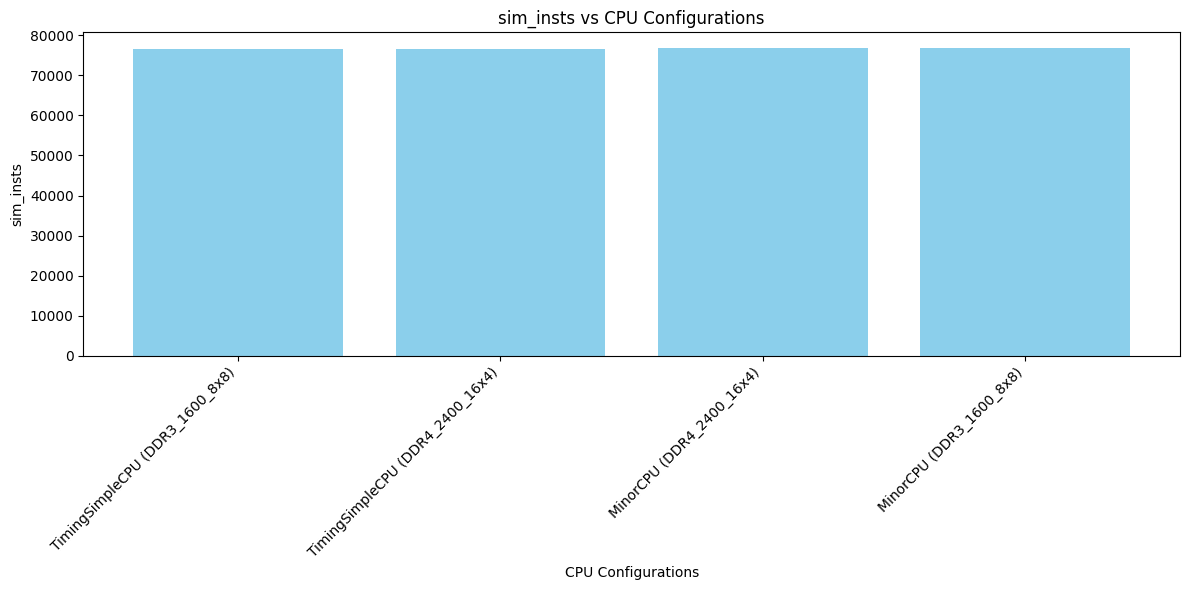
\includegraphics[width=16cm]{fib/fibonacci-charts.png}
    \caption{Simulated Instructions}
    \label{fig:enter-label}
\end{figure}

\begin{figure}[H]
    \centering
    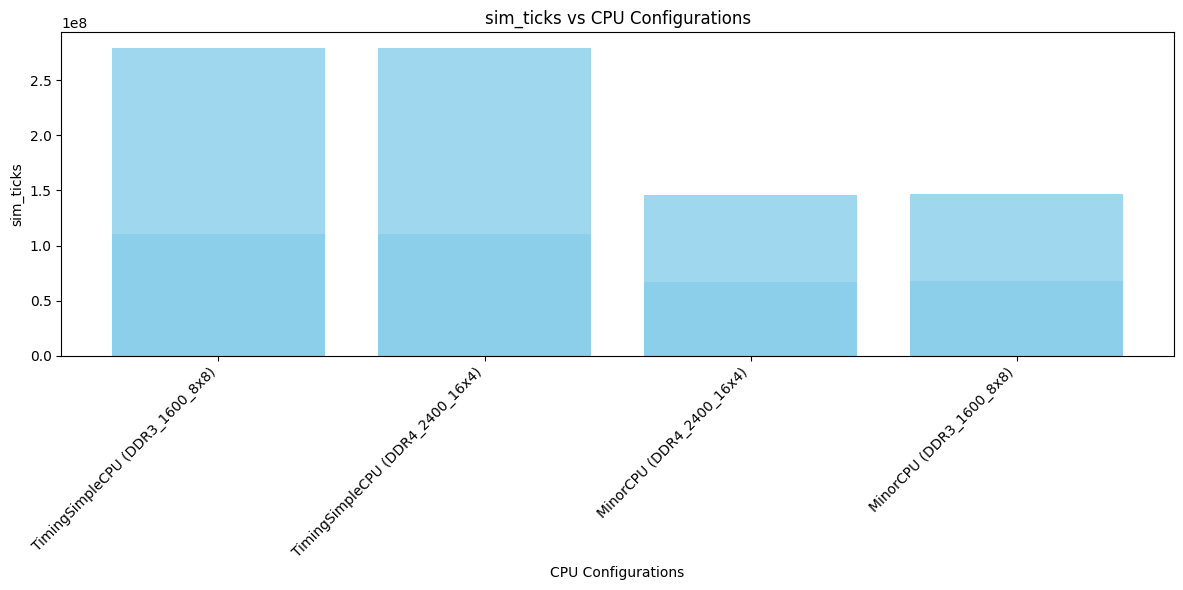
\includegraphics[width=16cm]{fib/fibonacci-charts-2.png}
    \caption{Simulated Ticks}
    \label{fig:enter-label}
\end{figure}

\begin{figure}[H]
    \centering
    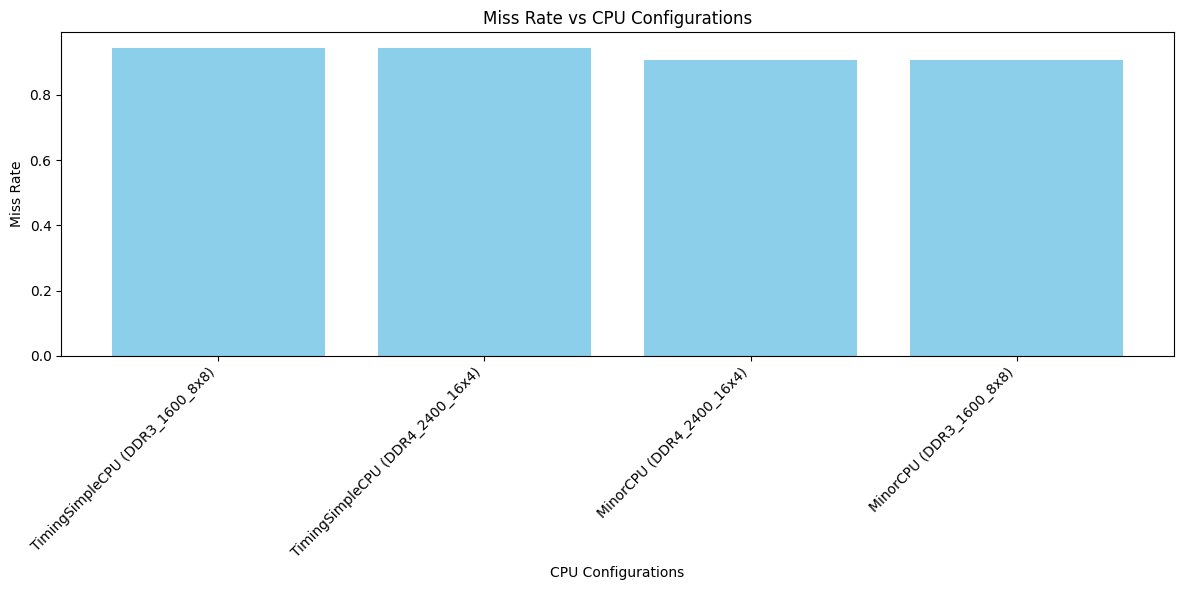
\includegraphics[width=16cm]{fib/fibonacci-charts-3.png}
    \caption{Miss Rate}
    \label{fig:enter-label}
\end{figure}

Παρατηρούμε ότι η αρχιτεκτονική του μοντέλου παίζει τον κυρίαρχο ρόλο και η τεχνολογία των μνημών επηρρεάζει σε ελάχιστο βαθμό. \\
Ο λόγος είναι ότι το (απλό) μοντέλο TimingSimpleCPU δεν χρησιμοποιεί pipelining ούτε speculative execution και γι'αυτό υστερεί. \\
Επίσης, παρατηρούμε ότι ότι τα sim\_ticks μειώνονται με την αύξηση του ρολογιού σε 3GHz αλλά δεν υποτριπλασιάζονται. \\
Κάποια components, όπως οι μνήμες, έχουν fixed latencies στον προσομοιωτή, συνεπώς δεν επηρεάζονται από την αύξηση του ρολογιού. \\
Ένας ακόμη λόγος που μπορεί να βλέπουμε πλήρη μείωση στα sim\_ticks είναι ότι σε πολύ γρήγορα συστήματα είναι σύνηθες φαινόμενο οι μνήμες να αποτελούν το bottleneck του συστήματος. \\
Τέλος, υπάρχει η πιθανότητα να εμφανιστούν ατέλειες στο pipeline (branch misspredictions, cache misses κλπ) όταν έχουμε ένα γρηγορότερο ρολόι κάτι που όμως διαπιστώνουμε ότι δεν συμβαίνει εδώ. \\

\section{Μέρος 2}
\subsection{}
\subsubsection{1}
Στο αρχείο Options.py μπορούμε να βρούμε τις ακόλουθες πληροφορίες σχετικά με τις (default) caches.

\begin{center}
\begin{tabular}{|c|c|c|c|}
 \hline
  & L2 & L1i & L1d \\
 Size & 2MB & 32kB & 64kB \\
 Associativity & 8 & 2 & 2 \\
 \hline
\end{tabular}
\end{center}
Η cache line έχει μέγεθος 64 bytes.\\ 

\subsubsection{2}

\begin{center}
\begin{tabular}{|c|c|c|c|c|c|}
 \hline
   & specbzip & spechmmer & speclibm & specmcf & specsjeng\\
 sim\_seconds & 0.083982 & 0.059396 & 0.174671 & 0.064955 & 0.513528\\
 CPI & 1.679650 & 1.187917 & 3.493415 & 1.299095 & 10.270554\\
 L1d Miss Rate & 0.014798 & 0.001637 & 0.060972 & 0.002108 & 0.121831 \\
 L1i Miss Rate & 0.000077 & 0.000221 & 0.000094 & 0.023612 & 0.000020 \\
 L2 Miss Rate & 0.282164 & 0.077760 & 0.999944 & 0.055046 & 0.999972\\
 \hline
\end{tabular}
\end{center}

\begin{figure}[H]
    \centering
    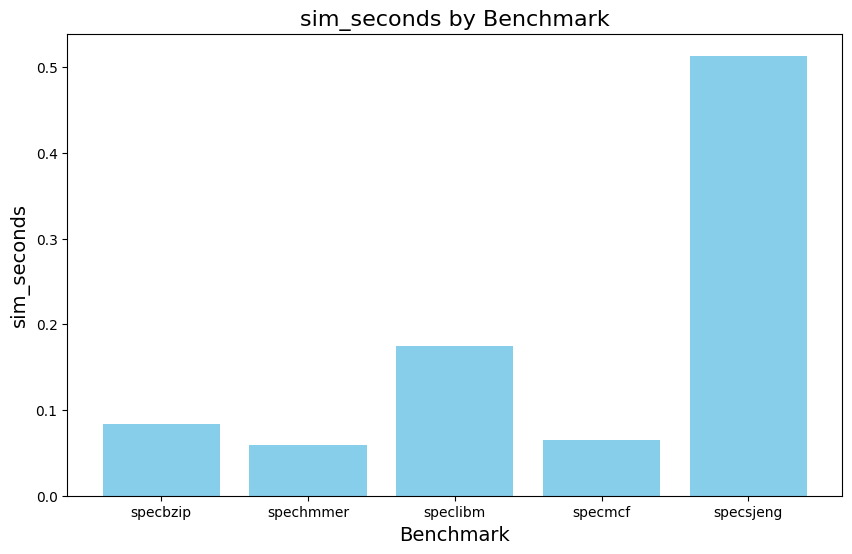
\includegraphics[width=16cm]{bench_metrics/sim_secs.png}
    \caption{Simulated Seconds}
    \label{fig:enter-label}
\end{figure}

\begin{figure}[H]
    \centering
    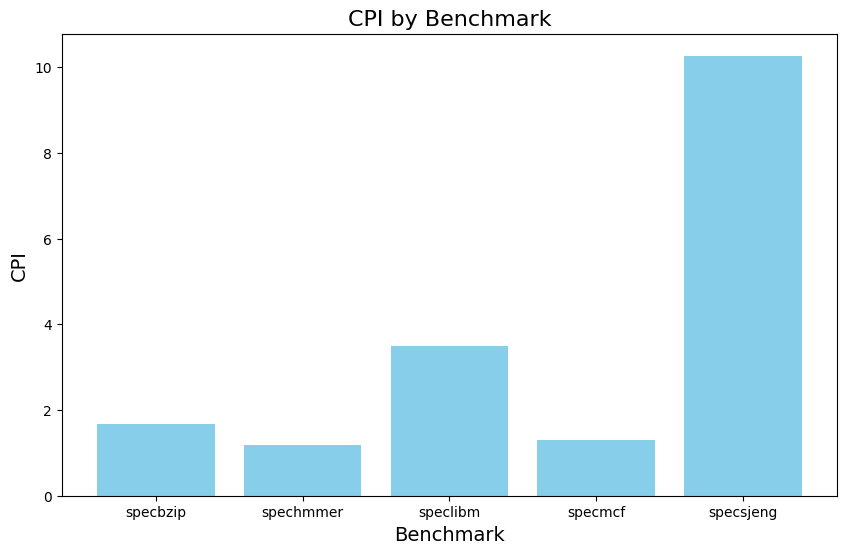
\includegraphics[width=16cm]{bench_metrics/cpi.png}
    \caption{CPI}
    \label{fig:enter-label}
\end{figure}

\begin{figure}[H]
    \centering
    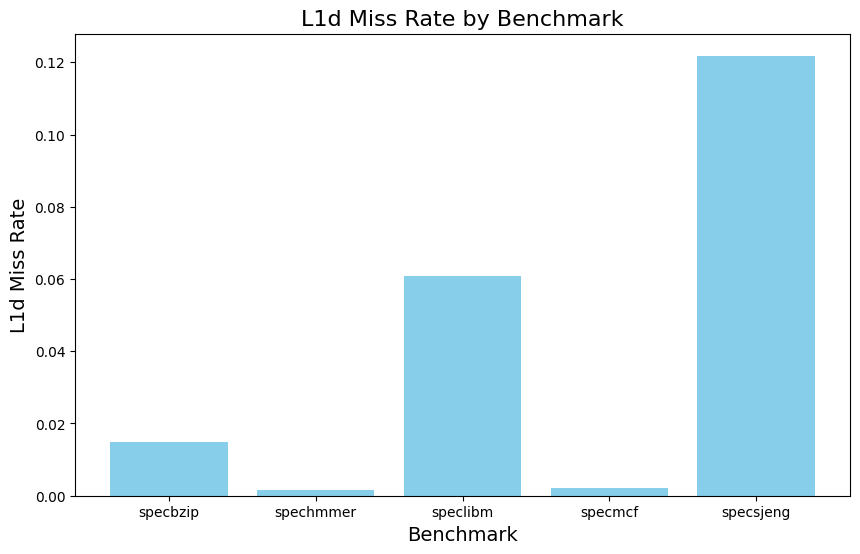
\includegraphics[width=16cm]{bench_metrics/l1d.png}
    \caption{L1d Miss Rate}
    \label{fig:enter-label}
\end{figure}

\begin{figure}[H]
    \centering
    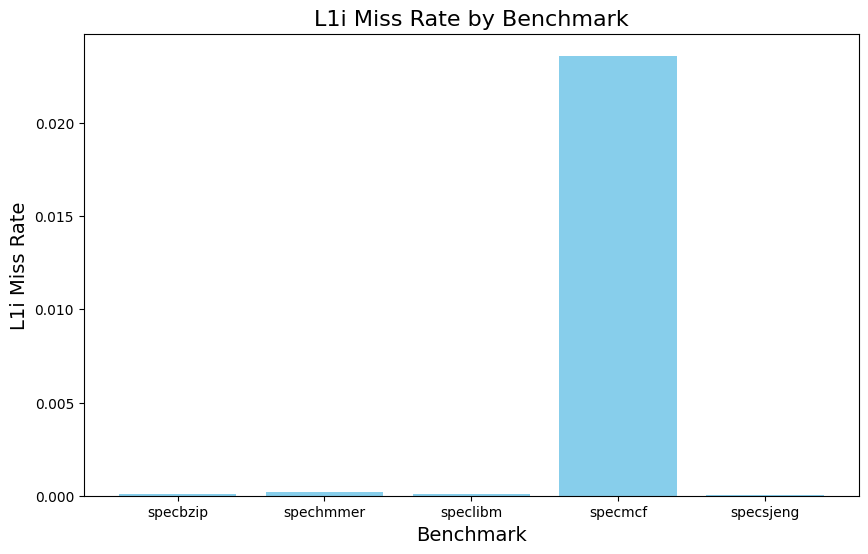
\includegraphics[width=16cm]{bench_metrics/l1i.png}
    \caption{L1i Miss Rate}
    \label{fig:enter-label}
\end{figure}

\begin{figure}[H]
    \centering
    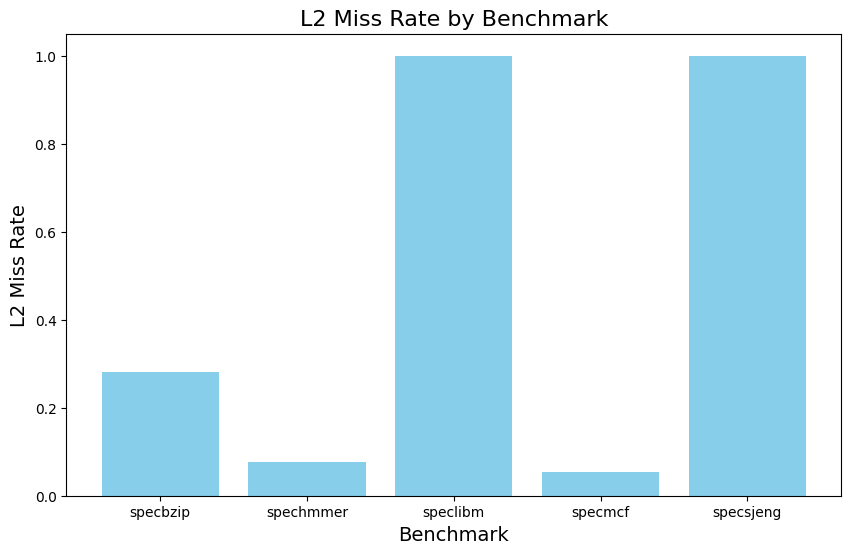
\includegraphics[width=16cm]{bench_metrics/l2.png}
    \caption{L2 Miss Rate}
    \label{fig:enter-label}
\end{figure}

Παρατηρούμε ότι το specsjeng είναι πιο σύνθετο με αποτέλεσμα να έχει πολύ μεγαλύτερο sim\_seconds, καθώς και CPI και L1d και L2 Miss Rates. \\
Το L1i Miss Rate του είναι χαμηλό, συνεπώς μπορούμε να καταλάβουμε ότι δεν υπάρχει καλό locality των δεδομένων. \\
Κάτι ακόμη που παρατηρούμε σχετικά με το specmcf είναι ότι έχει πολύ υψηλότερο L1i Miss Rate σε σχέση με τα υπόλοιπα benchmark, τα οποία είναι κοντά στο 0. \\
Αυτό μπορεί να συμβαίνει λόγω μεγάλου αποτυπώματος μνήμης εντολών τα οποία δεν χωράνε στην L1i, είτε λόγω κακού (spacial or temporal) locality στις εντολές. \\

\subsubsection{3}
\begin{center}
\begin{tabular}{|c|c|c|c|c|c|}
 \hline
   & specbzip & spechmmer & speclibm & specmcf & specsjeng\\
 (1GHz) sim\_seconds & 0.161025 & 0.262327 & 0.174671 & 0.127942 & 0.704056\\
 (3GHz) sim\_seconds & 0.039646 & 0.146433 & 0.146433 & 0.043867 & 0.449821\\
 \hline
\end{tabular}
\end{center}
Το σύστημα, ο CPU και οι μνήμες έχουν χρονιστεί στο 1GHz όπως διαπιστώνουμε από το config.json. \\
Χρονίζοντας το CPU στα 3GHz, τα υπόλοιπα παραμένουν στο 1GHz. \\
Εαν προσθέσουμε ακόμη ένα CPU θα είναι και αυτός χρονισμένος στα 3GHz, εκτός αν ορίσουμε εμείς κάποια άλλη επιθυμητή συχνότητα. \\
Παρατηρώντας τα αποτελέσματα βλέπουμε ότι δεν υπάρχει το ίδιο scaling για όλα τα benchmarks. \\
To specbzip για παράδειγμα έχει speedup 4x ενώ το speclibm έχει μόλις 1.19x. \\
Ο πιθανός λόγος είναι τα memory bottlenecks και πιθανώς ανεπάρκεια του pipeline να αξιοποιήσει πλήρως τα 3GHz (πχ. λόγω dependancies). \\ 
\subsubsection{4}
Επιλέγουμε το speclibm για να τρέξει με --mem-type=DDR3\_2133\_8x8. \\
Παρατηρούμε ότι sim\_seconds 0.171530 έναντι 0.174671, δηλαδή μία επιτάχυνση μικρότερη του 2\%. \\
Η επιλογή του συγκεκριμένου benchmark έγινε λόγω του μεγάλου (σχετικά) L2 Miss Rate με στόχο να αξιοποιηθεί η ταχύτητερα DDR3 ωστόσο η επιτάχυνση που πετύχαμε δεν ήταν η αναμενώμενη. \\
\end{document}